\documentclass[12pt, a4paper]{article}

% ==========================================
% 1. KHAI BÁO GÓI THƯ VIỆN (PACKAGES)
% ==========================================
% Bảng mã & Font chữ
\usepackage[utf8]{inputenc}
\usepackage[T5]{fontenc}

% Toán học
\usepackage{amsmath, amssymb}

% Căn lề & Bố cục trang
\usepackage[top=2.2cm, bottom=1.5cm, left=1cm, right=1cm, headheight=15pt]{geometry}
\usepackage{fancyhdr}
\usepackage{needspace}
\usepackage{tkz-tab}

% Đồ họa & Màu sắc
\usepackage{xcolor}
\usepackage{graphicx} 
\usepackage{tikz}
\usetikzlibrary{calc, shapes.geometric, positioning}


% Bảng biểu & Danh sách
\usepackage{colortbl}
\usepackage{array}
\usepackage{makecell}
\usepackage{multirow}
\usepackage{tasks}

% Biểu tượng
\usepackage{fontawesome5}

% ==========================================
% 2. THIẾT LẬP MÀU SẮC CHỦ ĐẠO
% ==========================================
\definecolor{goldyellow}{RGB}{255, 179, 0}
\definecolor{amberorange}{RGB}{230, 115, 0}
\definecolor{lightamber}{RGB}{255, 248, 225}
\definecolor{deepblue}{RGB}{25, 42, 86}
\definecolor{accentred}{RGB}{232, 65, 24}
\definecolor{softgray}{RGB}{220, 220, 222} 
\definecolor{fbblue}{RGB}{15, 80, 200}


% ==========================================
% 3. CẤU HÌNH HEADER & FOOTER
% ==========================================
\pagestyle{fancy}
\fancyhf{}
\renewcommand{\headrulewidth}{0pt}

% Khai báo biến lưu trữ nội dung góc phải của Header
\newcommand{\HeaderRightText}{}

% --- Header ---
\fancyhead[C]{
    \begin{tikzpicture}[remember picture, overlay]
        
        % Dải màu trang trí góc trên
        \path[fill=deepblue] (current page.north west) -- (current page.north east) 
            -- ($(current page.north east) + (0, -1.6cm)$) 
            .. controls ($(current page.north) + (3, -2.0cm)$) and ($(current page.north) + (-3, -0.4cm)$) .. 
            ($(current page.north west) + (0, -1.0cm)$) -- cycle;
            
        \path[fill=goldyellow] (current page.north west) -- (current page.north east) 
            -- ($(current page.north east) + (0, -1.0cm)$) 
            .. controls ($(current page.north) + (4, -1.0cm)$) and ($(current page.north) + (-2, -2.2cm)$) .. 
            ($(current page.north west) + (0, -1.6cm)$) -- cycle;
            
        \path[fill=amberorange] (current page.north west) -- ($(current page.north west) + (6.5cm, 0)$) 
            .. controls ($(current page.north west) + (4.5cm, -1.2cm)$) and ($(current page.north west) + (2cm, -2.0cm)$) .. 
            ($(current page.north west) + (0, -2.0cm)$) -- cycle;
            
        % Logo góc trái Header
        \node[anchor=west, inner sep=0pt] 
            at ($(current page.north west) + (0cm, -0.8cm)$) {
\includegraphics[height=2.0cm]{../image/logo-header.png}};
            
        % Text góc phải Header (Tự động lấy từ đối số thứ 3 của \titlebox)
        \node[anchor=east, text=white, font=\small\bfseries\sffamily] 
            at ($(current page.north east) + (-0.8cm, -0.5cm)$) {\HeaderRightText};
    \end{tikzpicture}
}

% --- Footer ---
\fancyfoot[C]{
    \begin{tikzpicture}[remember picture, overlay]
        % Đường kẻ ngang
        \draw[amberorange, line width=1.5pt] 
            ($(current page.south west) + (0cm, 0.4cm)$) -- ($(current page.south east) + (0cm, 0.4cm)$);

        % Dải cong góc phải
        \path[fill=goldyellow] (current page.south east) -- ($(current page.south east) + (-5cm, 0)$) 
            .. controls ($(current page.south east) + (-3cm, 0.8cm)$) and ($(current page.south east) + (-1.5cm, 1.2cm)$) .. 
            ($(current page.south east) + (0, 1.2cm)$) -- cycle;

        % Mạng xã hội
        \node[anchor=west, inner sep=0pt] at ($(current page.south west) + (1cm, 0.8cm)$) {
            \small\sffamily
            \textcolor{fbblue}{\faFacebook\hskip 4pt Toán Anh Huy MATH-STER}
            \hskip 18pt
            \textcolor{black}{\faTiktok\hskip 4pt huymathster}
        };

        % Số trang (Thiết kế hình tròn cũ thu nhỏ)
        \node[circle, fill=white, draw=amberorange, line width=1.5pt, text=deepblue, font=\large\bfseries, inner sep=0pt, minimum size=0.7cm] 
            at ($(current page.south east) + (-1.0cm, 0.65cm)$) {\thepage};
    \end{tikzpicture}
}

% ==========================================
% 4. ĐỊNH NGHĨA MACRO: KHUNG TIÊU ĐỀ
% ==========================================
\newcommand{\titlebox}[3]{
    % Gán nội dung đối số #3 vào biến HeaderRightText
    \gdef\HeaderRightText{#3}
    
    \begin{center}
    \vspace*{-0.5cm}
    \begin{tikzpicture}
        % Khung vô hình (Phantom Box) định chuẩn kích thước
        \node[text width=16cm, inner xsep=0pt, inner ysep=16pt, opacity=0] (MainBox) {
            \begin{minipage}[c]{4.2cm}
                \centering\vspace{0.1cm}
                \rule{2.2cm}{2.2cm} 
                \vspace{0.1cm}
            \end{minipage}%
            \begin{minipage}[c]{11.5cm}
                \centering\vspace{0.15cm}
                {\huge\bfseries\sffamily #2 \par}
                \vspace{0.15cm} 
            \end{minipage}
        };
        
        % Đổ bóng & Nền
        \fill[goldyellow, rounded corners=8pt] ([xshift=5pt, yshift=-5pt]MainBox.south west) rectangle ([xshift=5pt, yshift=-5pt]MainBox.north east);
        \fill[white, rounded corners=8pt] (MainBox.south west) rectangle (MainBox.north east);
        
        % Lưới ô ly & Nền Logo
        \begin{scope}
            \clip[rounded corners=8pt] (MainBox.south west) rectangle (MainBox.north east);
            \draw[step=0.4cm, softgray!50, line width=0.6pt] (MainBox.south west) grid (MainBox.north east);
            \fill[lightamber!60] (MainBox.south west) rectangle ([xshift=4.2cm]MainBox.north west);
        \end{scope}

        % Viền ngoài
        \draw[deepblue, line width=1.5pt, rounded corners=8pt] (MainBox.south west) rectangle (MainBox.north east);

        % Nội dung Text (Lớp trên cùng)
        \node[text width=16cm, inner xsep=0pt, inner ysep=16pt] at (MainBox.center) {
            \begin{minipage}[c]{4.2cm}
                \centering
                % --- ĐIỀU CHỈNH TỌA ĐỘ LOGO Ở ĐÂY ---
                \hspace*{-0.5cm}\raisebox{-0.2cm}{
\includegraphics[width=5.5cm]{../image/logo.png}}
            \end{minipage}%
            \begin{minipage}[c]{11.5cm}
                \centering\vspace{0.15cm}
                {\huge\bfseries\sffamily\color{deepblue} #2 \par}
                \vspace{0.15cm} 
            \end{minipage}
        };
        
        % Trang trí phụ kiện
        \draw[deepblue, line width=1.5pt, dashed] ([xshift=4.2cm]MainBox.north west) -- ([xshift=4.2cm]MainBox.south west);
        \node[regular polygon, regular polygon sides=4, rotate=45, fill=white, draw=accentred, line width=1.2pt, inner sep=2.5pt] at ([xshift=4.2cm]MainBox.west) {};
        \node[anchor=west, fill=amberorange, text=white, font=\large\bfseries\sffamily, rounded corners=4pt, draw=deepblue, line width=1.5pt, inner xsep=12pt, inner ysep=6pt] at ([xshift=1.5cm]MainBox.north west) {#1};
        \fill[accentred] ([xshift=-1.8cm, yshift=-0.4cm]MainBox.north east) circle (3pt);
        \fill[amberorange] ([xshift=-1.4cm, yshift=-0.4cm]MainBox.north east) circle (3pt);
        \fill[goldyellow] ([xshift=-1.0cm, yshift=-0.4cm]MainBox.north east) circle (3pt);
    \end{tikzpicture}
    \vspace*{0cm}
    \end{center}
}

% ==========================================
% 5. ĐỊNH NGHĨA MACRO: CẤU TRÚC CÂU HỎI (ÉP SÁT NHAU)
% ==========================================
\newcommand{\questioncore}[2]{
    % Xóa khoảng cách phía trên, ép sát câu trước
    \noindent \textbf{\textcolor{deepblue}{Câu #1.} \textcolor{accentred}{[STER]}} #2
    \par\nopagebreak
}

% Cấu hình hiển thị đáp án trắc nghiệm
\settasks{
    label=\textbf{\textcolor{amberorange}{\Alph*.}}, 
    label-width=15pt,     
    item-indent=25pt,     
    label-offset=6pt,    
    column-sep=20pt,     
    after-item-skip=2pt  % Đã giảm tối đa khoảng cách giữa các dòng đáp án A B C D
}

% Hàm vẽ dòng kẻ nháp
\newcommand{\drawdashlines}[1]{
    \ifnum#1>0
        \nopagebreak\vspace{0.1cm}\noindent 
        \begin{tikzpicture}
            \foreach \i in {1,...,#1} {
                \draw[softgray, line width=0.2pt] (0,-{\i*0.8}) -- (\textwidth-4pt,-{\i*0.8});
            }
        \end{tikzpicture}
        \par
    \fi
    % Đã xóa hoàn toàn khoảng cách thừa ở nhánh else
}

% --- Dạng 1: Trắc nghiệm 4 đáp án ---
\newcommand{\questionLinesManual}[4]{
    \pgfmathsetmacro{\calculatedSpace}{1.5 + #1 * 0.65}
    \needspace{\calculatedSpace cm} 
    \questioncore{#2}{#3}
    #4
    \par\nopagebreak
    \drawdashlines{#1}
}

\usepackage{cellspace}
\setlength\cellspacetoplimit{4pt}    % Khoảng đệm tự động phía trên ô
\setlength\cellspacebottomlimit{4pt} % Khoảng đệm tự động phía dưới ô




\newcommand{\questionTrueFalse}[4]{
    \scriptsize
    \pgfmathsetmacro{\calculatedSpace}{3.0 + #1 * 0.65} 
    \needspace{\calculatedSpace cm}
    \questioncore{#2}{#3}
    
    \nopagebreak
    \begin{flushleft}
     \renewcommand{\arraystretch}{1.2} % Bóp nhỏ chiều cao của bảng Đ/S
    \begin{tabular}{|>{\centering\arraybackslash}S{m{0.4cm}}|S{m{6cm}}|>{\centering\arraybackslash}S{m{1cm}}|>{\centering\arraybackslash}S{m{1cm}}|}
        \hline
        \rowcolor{amberorange!20}
        \multicolumn{1}{|c|}{} & \multicolumn{1}{>{\centering\arraybackslash}m{6cm}|}{\textbf{\textcolor{deepblue}{Mệnh đề}}} & 
        \textbf{\textcolor{deepblue}{Đúng}} & 
        \textbf{\textcolor{deepblue}{Sai}} \\
        \hline
        #4
        \hline
    \end{tabular}
    \renewcommand{\arraystretch}{1}
    \end{flushleft}
    
    \par\nopagebreak
    \drawdashlines{#1}
}

% ----- Dạng 3: Tự luận ngắn -----
\newcommand{\questionShortAnswer}[3]{
    \pgfmathsetmacro{\calculatedSpace}{1.5 + #1 * 0.8}
    \needspace{\calculatedSpace cm}
    
    {\linespread{1.1}\selectfont % Bóp nhỏ giãn dòng của câu tự luận
    \questioncore{#2}{#3}\par}
    
    \nopagebreak
    \begin{flushright}
        \begin{tikzpicture}
            \node[anchor=east, font=\small\bfseries\sffamily, text=deepblue] 
                at (-0.2, 0.4) {Đáp án:};
            \fill[goldyellow, rounded corners=3pt] (0.08, -0.08) rectangle (3.08, 0.72);
            \draw[draw=deepblue, fill=white, line width=1.2pt, rounded corners=3pt] 
                (0,0) rectangle (3.0, 0.8);
            \foreach \x in {0.75, 1.5, 2.25} {
                \draw[draw=deepblue, line width=0.6pt] (\x, 0) -- (\x, 0.8);
            }
        \end{tikzpicture}
    \end{flushright}
    
    \par\nopagebreak
    \drawdashlines{#1}
}


\settasks{
    after-item-skip = 1em % Tương đương row-skip cũ
}

% ==========================================
% BẮT ĐẦU NỘI DUNG TÀI LIỆU
% ==========================================
\begin{document}

% Truyền 3 tham số: {Nhãn cam} {Chữ to chính giữa} {Chữ ở góc phải Header}
\titlebox{Chủ đề: CTQ}{THPTQG 2026 LẦN 2}{THPTQG 2026: Chuyên Tuyên Quang}

\textit{Phần I: Thí sinh trả lời từ câu 1 đến câu 12, mỗi câu thí sinh chỉ chọn một phương án}

\vspace{0.5cm}

% --- CÂU 1 ---
\questionLinesManual{10}{1}{Phương trình \( \sin x = 0 \) có tập nghiệm là}{
    \begin{tasks}(2)
        \task \( S = \left\{ -\dfrac{\pi}{2} + k2\pi \,|\, k \in \mathbb{Z} \right\} \)
        \task \( S = \{k\pi \,|\, k \in \mathbb{Z}\} \)
        \task \( S = \{k2\pi \,|\, k \in \mathbb{Z}\} \)
        \task \( S = \left\{ \dfrac{\pi}{2} + k2\pi \,|\, k \in \mathbb{Z} \right\} \)
    \end{tasks}
}

% --- CÂU 2 ---
\questionLinesManual{5}{2}{Sau khi khảo sát về mức lượng khởi điểm (đơn vị: triệu đồng) của 20 công nhân, người ta thu được mẫu số liệu ghép nhóm như sau:}{
    \begin{center}
    \begin{tabular}{|c|c|c|c|c|c|c|}
        \hline
        Mức lượng & [5;6) & [6;7) & [7;8) & [8;9) & [9;10) & [10;11) \\
        \hline
        Tần số & 4 & 5 & 5 & 3 & 2 & 1 \\
        \hline
    \end{tabular}
    \end{center}
    Khoảng biến thiên của mẫu số liệu ghép nhóm đó bằng
    \begin{tasks}(4)
        \task \( 6 \)
        \task \( 1 \)
        \task \( 7,35 \)
        \task \( 1,42 \)
    \end{tasks}
}

% --- CÂU 3 ---
\questionLinesManual{5}{3}{Trong không gian với hệ tọa độ \( Oxyz \), phương trình của đường thẳng đi qua điểm \( A(1;3;-5) \) và có một vectơ chỉ phương \( \vec{u} = (2;-1;3) \) là}{
    \begin{tasks}(2)
        \task \( \dfrac{x-1}{2} = \dfrac{y+3}{-1} = \dfrac{z-5}{3} \)
        \task \( \dfrac{x-1}{2} = \dfrac{y+3}{-1} = \dfrac{z+5}{3} \)
        \task \( \dfrac{x-1}{2} = \dfrac{y-3}{-1} = \dfrac{z+5}{3} \)
        \task \( \dfrac{x-1}{2} = \dfrac{y-3}{-1} = \dfrac{z-5}{3} \)
    \end{tasks}
}

% --- CÂU 4 ---
\questionLinesManual{5}{4}{Cho hàm số \( f(x) \) liên tục trên \( \mathbb{R} \) có một nguyên hàm là \( F(x) \) thỏa mãn \( F(1) = 3, F(2) = 9 \). Phát biểu nào sau đây là đúng?}{
    \begin{tasks}(4)
        \task \( \displaystyle\int_1^2 f(x)dx = 12 \)
        \task \( \displaystyle\int_1^2 f(x)dx = 3 \)
        \task \( \displaystyle\int_1^2 f(x)dx = 6 \)
        \task \( \displaystyle\int_1^2 f(x)dx = 27 \)
    \end{tasks}
}

% --- CÂU 5 ---
\questionLinesManual{5}{5}{Cho hàm số \( y = f(x) = \dfrac{ax + 4}{3x + 1} \) (với \( a > 12 \)). Đạo hàm của hàm số đã cho là}{
    \begin{tasks}(4)
        \task \( y' = \dfrac{-a - 12}{(3x + 1)^2} \)
        \task \( y' = \dfrac{a - 12}{(3x + 1)^2} \)
        \task \( y' = \dfrac{a + 12}{(3x + 1)^2} \)
        \task \( y' = \dfrac{12 - a}{(3x + 1)^2} \)
    \end{tasks}
}

% --- CÂU 6 ---
\questionLinesManual{5}{6}{Cho hàm số \( f(x) = ax + b \) (\( a, b \in \mathbb{R}, a \neq 0 \)). Phát biểu nào sau đây là đúng?}{
    \begin{tasks}(2)
        \task \( \displaystyle\int 7f(x) dx = 7 + \int f(x) dx \)
        \task \( \displaystyle\int 7f(x) dx = 7 \int f(x) dx \)
        \task \( \displaystyle\int 7f(x) dx = 7 - \int f(x) dx \)
        \task \( \displaystyle\int 7f(x) dx = -7 \int f(x) dx \)
    \end{tasks}
}

% --- CÂU 7 ---
\questionLinesManual{3}{7}{Cho hàm số bậc ba \( y = f(x) \) có bảng biến thiên trên đoạn \([-1;2]\) như sau:
\begin{center}
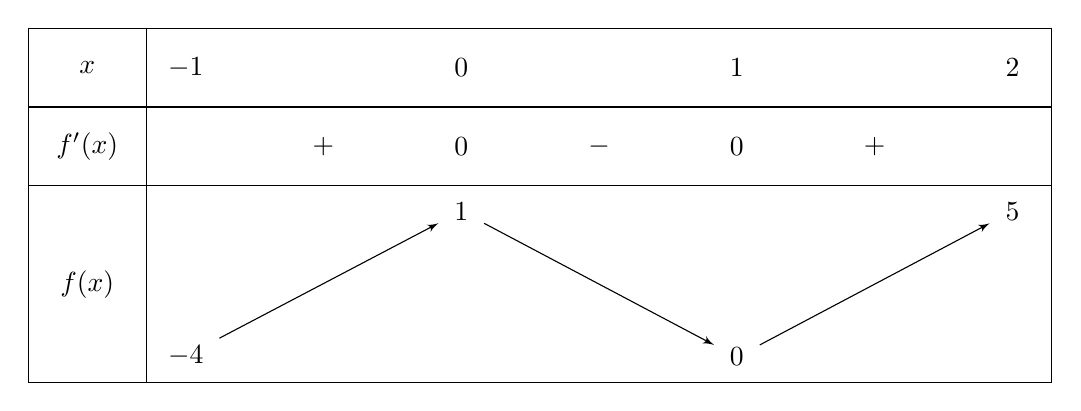
\begin{tikzpicture}
\tkzTabInit[color, lgt=1.5, espcl=3.5]
{$x$ / 1, $f'(x)$ / 1, $f(x)$ / 2.5}
{$-1$, $0$, $1$, $2$}
\tkzTabLine{ , +, 0, -, 0, + }
\tkzTabVar{-/$-4$, +/$1$, -/$0$, +/$5$}
\end{tikzpicture}
\end{center}
Giá trị lớn nhất của hàm số đã cho trên đoạn \([-1;2]\) bằng}{
    \begin{tasks}(4)
        \task \( 1 \)
        \task \( 5 \)
        \task \( 0 \)
        \task \( -4 \)
    \end{tasks}
}

% --- CÂU 8 ---
\questionLinesManual{3}{8}{Cho mẫu số liệu ghép nhóm về số giờ xem truyền hình của một nhóm học sinh như sau:
\begin{center}
\begin{tabular}{|c|c|c|c|c|c|}
\hline
Số giờ xem truyền hình & [0;2) & [2;4) & [4;6) & [6;8) & [8;10) \\
\hline
Tần số & 20 & 35 & 30 & 10 & 5 \\
\hline
\end{tabular}
\end{center}
Giá trị trung bình của mẫu số liệu ghép nhóm đó bằng (làm tròn kết quả đến hàng phần mười)}{
\begin{tasks}(2)
\task \( 3,9 \)
\task \( 4,6 \)
\task \( 2,1 \)
\task \( 10 \)
\end{tasks}
}

% --- CÂU 9 ---
\questionLinesManual{3}{9}{Cho hình hộp \(ABCD.A'B'C'D'\) (xem hình minh họa bên dưới). Vectơ nào sau đây cùng phương với vectơ \(\overrightarrow{A'D'}\)?}{
    \begin{center}
    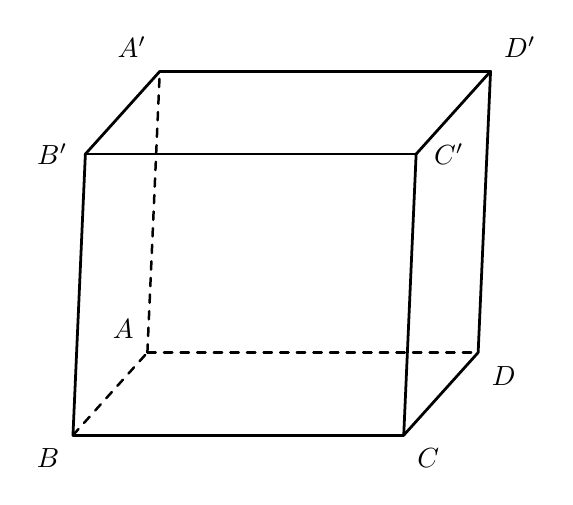
\begin{tikzpicture}[scale=1.05, line join=round, line cap=round]

        % =========================
        % TỌA ĐỘ CÁC ĐỈNH
        % =========================
        \coordinate (B)  at (0,0);
        \coordinate (C)  at (4,0);
        \coordinate (A)  at (0.9,1.0);
        \coordinate (D)  at (4.9,1.0);

        \coordinate (B') at (0.15,3.4);
        \coordinate (C') at (4.15,3.4);
        \coordinate (A') at (1.05,4.4);
        \coordinate (D') at (5.05,4.4);

        % =========================
        % CÁC CẠNH KHUẤT - NÉT ĐỨT
        % =========================
        \draw[dashed, line width=0.9pt]
            (B) -- (A);

        \draw[dashed, line width=0.9pt]
            (A) -- (D);

        \draw[dashed, line width=0.9pt]
            (A) -- (A');

        % =========================
        % CÁC CẠNH HIỆN - NÉT LIỀN
        % =========================

        % Đáy
        \draw[line width=1pt]
            (B) -- (C);

        \draw[line width=1pt]
            (C) -- (D);

        % Mặt trước
        \draw[line width=1pt]
            (B) -- (B');

        \draw[line width=1pt]
            (C) -- (C');

        \draw[line width=1pt]
            (B') -- (C');

        % Mặt trên
        \draw[line width=1pt]
            (B') -- (A');

        \draw[line width=1pt]
            (A') -- (D');

        \draw[line width=1pt]
            (C') -- (D');

        % Cạnh bên phải
        \draw[line width=1pt]
            (D) -- (D');

        % =========================
        % NHÃN CÁC ĐỈNH
        % =========================

        \node[below left=2pt]  at (B)  {\(B\)};
        \node[below right=2pt] at (C)  {\(C\)};
        \node[above left=2pt]  at (A)  {\(A\)};
        \node[below right=2pt] at (D)  {\(D\)};

        \node[left=3pt]  at (B') {\(B'\)};
        \node[right=3pt] at (C') {\(C'\)};
        \node[above left=2pt] at (A') {\(A'\)};
        \node[above right=2pt] at (D') {\(D'\)};

    \end{tikzpicture}
    \end{center}

    \begin{tasks}(4)
        \task \(\overrightarrow{BD}\)
        \task \(\overrightarrow{AB}\)
        \task \(\overrightarrow{AC}\)
        \task \(\overrightarrow{AD}\)
    \end{tasks}
}


% --- CÂU 10 ---
\questionLinesManual{5}{10}{Cho cấp số nhân \((u_n)\) có công bội \(q\) với \(u_1=m\) và \(u_2=n\), trong đó \(m>2,n>2m\). Phát biểu nào sau đây là đúng?}{
    \begin{tasks}(4)
        \task \(n=mq\)
        \task \(m=n+q\)
        \task \(m=nq\)
        \task \(n=m+q\)
    \end{tasks}
}


% --- CÂU 11 ---
\questionLinesManual{8}{11}{Cho hình chóp \(S.ABCD\) có đáy \(ABCD\) là hình vuông và \(SA\) vuông góc với \((ABCD)\). Đường thẳng \(BC\) vuông góc với mặt phẳng nào trong các mặt phẳng sau đây?}{
    \begin{center}
    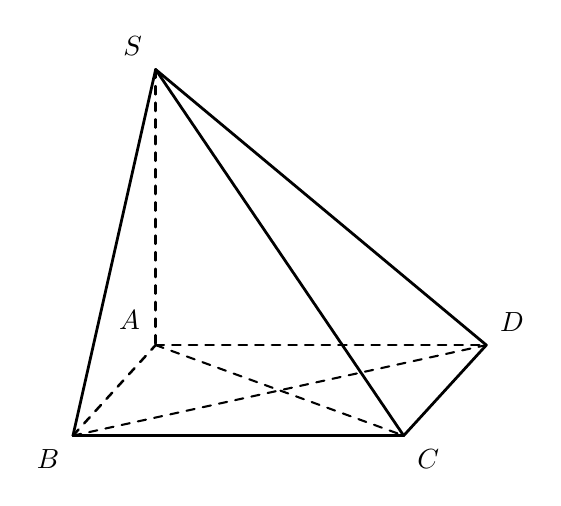
\begin{tikzpicture}[
        x=1cm,
        y=1cm,
        line join=round,
        line cap=round
    ]

        % =================================
        % TỌA ĐỘ CÁC ĐỈNH
        % =================================
        \coordinate (B) at (0,0);
        \coordinate (C) at (4.2,0);
        \coordinate (A) at (1.05,1.15);
        \coordinate (D) at (5.25,1.15);

        % Đỉnh S nằm trên A
        \coordinate (S) at (1.05,4.65);


        % =================================
        % ĐÁY ABCD
        % =================================

        % AB - cạnh khuất
        \draw[dashed, line width=0.9pt]
            (B) -- (A);

        % AD - cạnh khuất
        \draw[dashed, line width=0.9pt]
            (A) -- (D);

        % BC - cạnh trước
        \draw[line width=1pt]
            (B) -- (C);

        % CD - cạnh bên
        \draw[line width=1pt]
            (C) -- (D);


        % =================================
        % ĐƯỜNG CHÉO ĐÁY
        % =================================

        % AC
        \draw[dashed, line width=0.75pt]
            (A) -- (C);

        % BD
        \draw[dashed, line width=0.75pt]
            (B) -- (D);


        % =================================
        % CÁC CẠNH HÌNH CHÓP
        % =================================

        % SA - cạnh khuất
        \draw[dashed, line width=0.9pt]
            (S) -- (A);

        % SB
        \draw[line width=1pt]
            (S) -- (B);

        % SC
        \draw[line width=1pt]
            (S) -- (C);

        % SD
        \draw[line width=1pt]
            (S) -- (D);


        % =================================
        % NHÃN ĐỈNH
        % =================================

        \node[above left=2pt] at (S) {\(S\)};
        \node[above left=3pt] at (A) {\(A\)};
        \node[below left=2pt] at (B) {\(B\)};
        \node[below right=2pt] at (C) {\(C\)};
        \node[above right=2pt] at (D) {\(D\)};

    \end{tikzpicture}
    \end{center}

    \begin{tasks}(4)
        \task \((SCD)\)
        \task \((SAB)\)
        \task \((SBC)\)
        \task \((SBD)\)
    \end{tasks}
}

% --- CÂU 12 ---
\questionLinesManual{6}{12}{Nguyên hàm của hàm số \(f(x)=3x^2-\cos x\) là}{
    \begin{tasks}(4)
        \task \(x^3+\sin x+C\)
        \task \(6x+\sin x+C\)
        \task \(6x-\sin x+C\)
        \task \(x^3-\sin x+C\)
    \end{tasks}
}


% ==========================================
% PHẦN II: ĐÚNG - SAI
% ==========================================

\textit{\textbf{Phần II:} Thí sinh trả lời từ câu 1 đến câu 4; trong mỗi ý a), b), c), d) ở mỗi câu, thí sinh chọn đúng hoặc sai.}

\vspace{0.3cm}

% --- CÂU 1 PHẦN II ---
\questionTrueFalse{23}{1}{Cho hàm số \(y=f(x)=x^3-6x^2+9x+2\).}{
    \textbf{a)} & Đạo hàm của hàm số đã cho là \(f'(x)=3x^2-12x+9\).
    & \textcolor{amberorange}{$\bigcirc$} & \textcolor{amberorange}{$\bigcirc$} \\ \hline

    \textbf{b)} & Phương trình \(f'(x)=0\) có tập nghiệm là \(S=\{1;3\}\).
    & \textcolor{amberorange}{$\bigcirc$} & \textcolor{amberorange}{$\bigcirc$} \\ \hline

    \textbf{c)} & Hàm số đã cho đạt giá trị lớn nhất trên đoạn \([2;4]\) tại \(x=2\).
    & \textcolor{amberorange}{$\bigcirc$} & \textcolor{amberorange}{$\bigcirc$} \\ \hline

    \textbf{d)} & Gọi \(x_1,x_2\) là hai điểm cực trị của hàm số \(y=f(x)\). Khi đó, phương trình đường thẳng đi qua hai điểm
    \(M_1(x_1;f(x_1))\) và \(M_2(x_2;f(x_2))\) là \(y=-2x+1\).
    & \textcolor{amberorange}{$\bigcirc$} & \textcolor{amberorange}{$\bigcirc$} \\
}



% --- CÂU 2 PHẦN II ---
\questionTrueFalse{15}{2}{Người ta dùng một thiết bị bơm nước vào một bể không có nước. Tính từ lúc thiết bị bắt đầu hoạt động, tại thời điểm \(t\) giờ với \(0 \le t \le 8\), thiết bị đó có tốc độ bơm nước vào bể là \(f(t)\) (\(\text{m}^3\text{/giờ}\)). Biết rằng đồ thị của hàm số \(y = f(t)\) là một phần đường parabol đi qua gốc tọa độ \(O\) và hai điểm \(A(2;3)\), \(B(6;3)\) (xem hình minh họa bên dưới).
\begin{center}
\begin{tikzpicture}[scale=0.85, line join=round, line cap=round, >=stealth]
    % Trục tọa độ
    \draw[->, line width=0.8pt] (-0.8,0) -- (8.5,0) node[below] {\small \(t(\text{giờ})\)};
    \draw[->, line width=0.8pt] (0,-0.8) -- (0,4.8) node[left] {\small \(y = f(t)\)};
    \node[below left] at (0,0) {\small \(O\)};

    % Đồ thị Parabol y = 2t - 0.25 t^2
    \draw[line width=1.2pt, color=deepblue, domain=0:8, samples=100] 
        plot (\x, {2*\x - 0.25*\x*\x});

    % Điểm và đường dóng
    \draw[dashed, line width=0.6pt] (0,3) node[left] {\small \(3\)} -- (6,3);
    \draw[dashed, line width=0.6pt] (2,0) node[below] {\small \(2\)} -- (2,3);
    \draw[dashed, line width=0.6pt] (6,0) node[below] {\small \(6\)} -- (6,3);

    % Tọa độ các điểm A, B
    \fill[deepblue] (2,3) circle (2pt) node[above left] {\small \(A\)};
    \fill[deepblue] (6,3) circle (2pt) node[above right] {\small \(B\)};
\end{tikzpicture}
\end{center}
}{
    \textbf{a)} & Với \(0 \le t \le 8\) thì \(f(t) = 3t - \dfrac{t^2}{6}\) (\(\text{m}^3\text{/giờ}\)).
    & \textcolor{amberorange}{$\bigcirc$} & \textcolor{amberorange}{$\bigcirc$} \\ \hline

    \textbf{b)} & Tại thời điểm \(t\) giờ (\(0 \le t \le 8\)) tính từ lúc thiết bị bắt đầu hoạt động, lượng nước trong bể là \(V(t) = t^2 - \dfrac{t^3}{12}\) (\(\text{m}^3\)).
    & \textcolor{amberorange}{$\bigcirc$} & \textcolor{amberorange}{$\bigcirc$} \\ \hline

    \textbf{c)} & Tại thời điểm thiết bị có tốc độ bơm nước vào bể là lớn nhất, lượng nước trong bể lớn hơn \(10{,}7\) mét khối.
    & \textcolor{amberorange}{$\bigcirc$} & \textcolor{amberorange}{$\bigcirc$} \\ \hline

    \textbf{d)} & Sau \(\dfrac{a}{b}\) giờ tính từ lúc thiết bị bắt đầu hoạt động (trong đó \(\dfrac{a}{b}\) là phân số tối giản và \(b > 0\)), lượng nước trong bể là \(13{,}824\) mét khối. Khi đó, giá trị của \(a + b\) là \(29\).
    & \textcolor{amberorange}{$\bigcirc$} & \textcolor{amberorange}{$\bigcirc$} \\
}


% --- CÂU 3 PHẦN II ---
\questionTrueFalse{20}{3}{Trong không gian với hệ tọa độ \(Oxyz\), một trạm thu phát sóng điện thoại di động được đặt ở vị trí \(I(2;1;12)\), trong đó một đơn vị độ dài trên mỗi trục tương ứng với \(10\text{ mét}\) trên thực tế. Trạm thu phát sóng đó có bán kính phủ sóng là \(130\text{ mét}\). Vùng phủ sóng của trạm thu phát được quy ước là tập hợp tất cả các điểm \(P\) trên mặt đất và trong không gian sao cho khoảng cách \(IP\) không vượt quá \(130\text{ mét}\). Mặt đất được coi là một phần của mặt phẳng \((Oxy)\) và mỗi người trên mặt đất được coi như một chất điểm.}{
    \textbf{a)} & Vùng phủ sóng của trạm thu phát là một phần của hình cầu giới hạn bởi mặt cầu \((S)\) có phương trình \((x-2)^2 + (y-1)^2 + (z-12)^2 = 169\).
    & \textcolor{amberorange}{$\bigcirc$} & \textcolor{amberorange}{$\bigcirc$} \\ \hline

    \textbf{b)} & Giả sử một người cầm điện thoại đang ở vị trí điểm \(M(3;1;0)\) và chuyển động thẳng đều trên mặt đất với tốc độ \(3{,}6\text{ km/h}\). Khi đó, tại giây thứ \(40\) tính từ lúc xuất phát ở vị trí điểm \(M(3;1;0)\), người đó đã đi ra ngoài vùng phủ sóng của trạm thu phát.
    & \textcolor{amberorange}{$\bigcirc$} & \textcolor{amberorange}{$\bigcirc$} \\ \hline

    \textbf{c)} & Khoảng cách ngắn nhất để một người cầm điện thoại đang ở vị trí có tọa độ \(N(8;9;0)\) di chuyển trên mặt đất tới được vùng phủ sóng (theo đơn vị mét) là \(100\text{ m}\).
    & \textcolor{amberorange}{$\bigcirc$} & \textcolor{amberorange}{$\bigcirc$} \\ \hline

    \textbf{d)} & Giả sử một người cầm điện thoại chuyển động thẳng đều trên mặt đất từ vị trí \(A(6;9;0)\) đến vị trí \(B(-4;b;0)\) với tốc độ \(3{,}6\text{ km/h}\) sao cho khoảng thời gian người đó thuộc vùng phủ sóng đúng bằng \(60\text{ giây}\). Khi đó \(b = \dfrac{3}{2}\).
    & \textcolor{amberorange}{$\bigcirc$} & \textcolor{amberorange}{$\bigcirc$} \\
}

% --- CÂU 4 PHẦN II ---
\questionTrueFalse{24}{4}{Một trường đại học trao hai loại học bổng A và B cho sinh viên trong trường, một sinh viên có thể được nhận cả hai loại học bổng A và B. Trong số các sinh viên được trao học bổng loại A có \(12\%\) số bạn được trao học bổng loại B và trong số các sinh viên không được trao học bổng loại A có \(10\%\) số bạn được trao học bổng loại B. Có \(10{,}2\%\) số sinh viên toàn trường được trao học bổng loại B. Chọn ngẫu nhiên một sinh viên trong trường.}{
    \textbf{a)} & Xác suất để sinh viên đó không được trao học bổng loại B là \(0{,}898\).
    & \textcolor{amberorange}{$\bigcirc$} & \textcolor{amberorange}{$\bigcirc$} \\ \hline

    \textbf{b)} & Xác suất để sinh viên đó không được trao học bổng loại B, biết sinh viên đó không được trao học bổng loại A, là \(0{,}88\).
    & \textcolor{amberorange}{$\bigcirc$} & \textcolor{amberorange}{$\bigcirc$} \\ \hline

    \textbf{c)} & Xác suất để sinh viên đó không được trao học bổng loại A là \(0{,}89\).
    & \textcolor{amberorange}{$\bigcirc$} & \textcolor{amberorange}{$\bigcirc$} \\ \hline

    \textbf{d)} & Xác suất để sinh viên đó không được trao học bổng loại A, biết sinh viên đó không được trao học bổng loại B, lớn hơn \(0{,}9\).
    & \textcolor{amberorange}{$\bigcirc$} & \textcolor{amberorange}{$\bigcirc$} \\
}

% ==========================================
% PHẦN III: TRẢ LỜI NGẮN
% ==========================================

\textit{\textbf{Phần III:} Thí sinh trả lời từ câu 1 đến câu 6.}

\vspace{0.3cm}

% --- CÂU 1 PHẦN III ---
\questionShortAnswer{0}{1}{Cho bảng \(6 \times 6\) gồm \(36\) ô vuông đơn vị và cho \(8\) quân cờ đôi một khác nhau. Người ta xếp ngẫu nhiên \(8\) quân cờ đó vào \(36\) ô trong bảng sao cho mỗi ô xếp nhiều nhất một quân cờ. Hai cách xếp được gọi là như nhau nếu vị trí của \(8\) quân cờ tương ứng trên bảng là giống nhau sau khi xếp xong (không tính đến thứ tự xếp các quân cờ vào bảng). Chọn ngẫu nhiên một cách xếp như trên. Gọi \(P\) là xác suất của biến cố:

``Cách xếp được chọn thỏa mãn đồng thời ba điều kiện sau:
\begin{itemize}
    \item Trên mỗi hàng có ít nhất một quân cờ;
    \item Trên mỗi cột có ít nhất một quân cờ;
    \item Mỗi quân cờ phải cùng hàng với đúng một quân cờ khác hoặc cùng cột với đúng một quân cờ khác.''
\end{itemize}
Giá trị của \(9^4 P\) bằng bao nhiêu (không làm tròn kết quả các phép tính trung gian, chỉ làm tròn kết quả phép tính cuối cùng đến hàng phần trăm)?
\begin{center}

\begin{tikzpicture}
    \draw[step=1, thick] (0,0) grid (6,6);
    \draw[step=1, thick] (8,0) grid (14,6);
\end{tikzpicture}
\end{center}}

\drawdashlines{10}
\newpage
\drawdashlines{30}

% --- CÂU 2 PHẦN III ---
\questionShortAnswer{25}{2}{Công ty vận tải nhận một đơn hàng vận chuyển ít nhất \(23\) tấn hàng loại A, ít nhất \(59\) tấn hàng loại B và không quá \(139\) tấn hàng loại C. Công ty vận tải sử dụng hai loại xe X và Y để chở số hàng đó. Mỗi xe loại X đều chở \(12\) tấn hàng loại A, \(6\) tấn hàng loại B và \(18\) tấn hàng loại C. Mỗi xe loại Y đều chở \(2\) tấn hàng loại A, \(20\) tấn hàng loại B và \(22\) tấn hàng loại C. Chi phí cho \(1\) xe loại X là \(37\) triệu đồng và cho \(1\) xe loại Y là \(45\) triệu đồng. Gọi \(T\) (triệu đồng) là chi phí nhỏ nhất để công ty hoàn thành đơn hàng. Giá trị của \(10T\) bằng bao nhiêu?}

% --- CÂU 3 PHẦN III ---
\questionShortAnswer{23}{3}{Người ta cần tính thể tích của một vật thể được chế tác như sau. Trên mặt phẳng với hệ tọa độ \(Oxy\) (một đơn vị độ dài trên mỗi trục tương ứng với một xăng-ti-mét trong thực tế), gọi \((H)\) là hình phẳng được tô đậm, giới hạn bởi đường elip \(\dfrac{x^2}{256} + \dfrac{y^2}{48} = 1\) và đường tròn tâm \(O\) có bán kính \(10\) (xem hình minh họa bên dưới). Vật thể có dạng khối tròn xoay được tạo thành khi quay hình phẳng \((H)\) quanh trục hoành. Thể tích của vật thể nói trên bằng bao nhiêu xăng-ti-mét khối\linebreak (không làm tròn kết quả các phép tính trung gian, chỉ làm tròn kết quả phép tính cuối cùng đến hàng đơn vị)?

\begin{center}
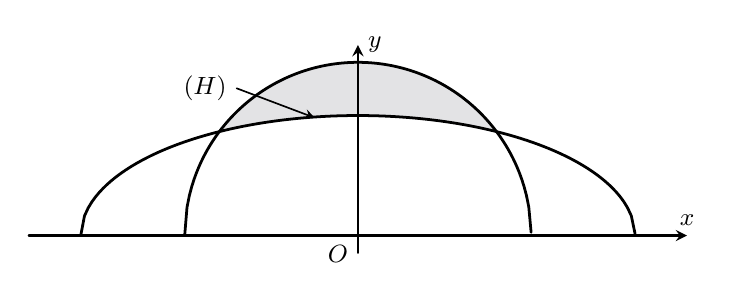
\begin{tikzpicture}[scale=0.22, line join=round, line cap=round, >=stealth]
    % Tọa độ Elip: a = 16, b = 4*sqrt(3) ≈ 6.928
    % Đường tròn: R = 10
    
    % Miền tô đậm (H): giới hạn phía trên bởi Elip, phía dưới bởi đường tròn, y >= 0
    % Giao điểm giữa elip y = sqrt(48*(1 - x^2/256)) và đường tròn y = sqrt(100 - x^2)
    % x^2/256 + (100 - x^2)/48 = 1 => 3x^2 + 16(100 - x^2) = 768 => 13x^2 = 832 => x^2 = 64 => x = ±8
    \begin{scope}
        \clip (-8, 6) -- (-8, 12) -- (8, 12) -- (8, 6) -- cycle;
        % Tô màu miền H
        \fill[softgray!80] 
            plot[domain=-8:8, samples=100] (\x, {sqrt(48*(1 - (\x)^2/256))}) 
            -- plot[domain=8:-8, samples=100] (\x, {sqrt(100 - (\x)^2)}) 
            -- cycle;
    \end{scope}

    % Trục tọa độ Oxy
    \draw[->, line width=0.8pt] (-19,0) -- (19,0) node[above] {\small \(x\)};
    \draw[->, line width=0.8pt] (0,-1) -- (0,11) node[right] {\small \(y\)};
    \node[below left] at (0,0) {\small \(O\)};

    % Vẽ nửa trên Elip
    \draw[line width=1.0pt, domain=-16:16, samples=150] 
        plot (\x, {sqrt(48*(1 - (\x)^2/256))});

    % Vẽ nửa trên đường tròn
    \draw[line width=1.0pt, domain=-10:10, samples=150] 
        plot (\x, {sqrt(100 - (\x)^2)});

    % Mũi tên chỉ miền (H)
    \draw[->, line width=0.6pt] (-7,8.5) node[left] {\small \((H)\)} -- (-2.5,6.8);
\end{tikzpicture}
\end{center}
}

% --- CÂU 4 PHẦN III ---
\questionShortAnswer{0}{4}{Cho bảng \(5 \times 5\) gồm \(25\) ô vuông đơn vị và cho bốn màu. Người ta tô mỗi ô trong bảng bởi một trong bốn màu đã cho sao cho hai ô bất kì có chung đỉnh hoặc chung cạnh thì khác màu. Hai cách tô màu bảng được gọi là giống nhau nếu mỗi ô của bảng có cùng màu ở cả hai cách tô (không tính đến thứ tự tô màu các ô). Gọi \(S\) là số cách tô màu bảng phân biệt thỏa mãn điều kiện trên. Giá trị của \(9S\) bằng bao nhiêu?
\begin{center}


\begin{tikzpicture}
    \draw[step=1, thick] (0,0) grid (5,5);
    \draw[step=1,  thick] (8,0) grid (13,5);
\end{tikzpicture}
\end{center}}

\drawdashlines{22}
\newpage
\drawdashlines{30}
% --- CÂU 5 PHẦN III ---
\questionShortAnswer{25}{5}{Một doanh nghiệp dự kiến sản xuất không quá \(2000\) sản phẩm cùng loại. Giả sử rằng doanh thu của doanh nghiệp khi sản xuất \(x\) sản phẩm (\(x \in \mathbb{N}; 0 \le x \le 2000\)) là \(R(x) = 16x - 0{,}005x^2\) (triệu đồng) và doanh nghiệp phải nộp một khoản thuế là \(5\%\) của doanh thu \(R(x)\). Chi phí để sản xuất mỗi sản phẩm là bốn triệu đồng. Lợi nhuận của doanh nghiệp (khi sản xuất \(x\) sản phẩm) được tính theo công thức: Lợi nhuận bằng doanh thu trừ đi thuế và chi phí. Doanh nghiệp phải sản xuất bao nhiêu sản phẩm để thu được lợi nhuận lớn nhất?}

% --- CÂU 6 PHẦN III ---
\questionShortAnswer{25}{6}{Cho tứ diện \(ABCD\) có \(AB = CD = 20\sqrt{5}\), \(AC = BD = 50\), \(AD = BC = 10\sqrt{13}\). Thể tích của khối tứ diện đã cho bằng bao nhiêu?}

% --- DÒNG KẺ HẾT ---
\begin{center}
    \begin{tikzpicture}
        \draw[deepblue, line width=1.2pt] (-4,0) -- (-0.8,0);
        \node[font=\bfseries\sffamily, text=accentred] at (0,0) {HẾT};
        \draw[deepblue, line width=1.2pt] (0.8,0) -- (4,0);
    \end{tikzpicture}
\end{center}

% --- KHUNG LƯU Ý CẢNH BÁO ĐỎ ---
\begin{center}
\begin{tikzpicture}
    % Khung nền viền đứt đôi
    \draw[accentred, line width=1.8pt, fill=accentred!8, rounded corners=10pt] 
        (0,0) rectangle (13, 1.6);
    \draw[amberorange, line width=0.8pt, dashed, rounded corners=8pt] 
        (0.08, 0.08) rectangle (12.92, 1.52);
        
    % Icon chuông / cảnh báo lớn ở góc trái
    \node[circle, fill=accentred, text=white, inner sep=6pt] at (0.8, 0.8) {\Large\faBell};

    % Đường ngăn cách dọc
    \draw[accentred!50, line width=1pt] (1.5, 0.2) -- (1.5, 1.4);

    % Nội dung chữ
    \node[anchor=west, text width=10.8cm, font=\large\bfseries\sffamily\color{deepblue}] at (1.8, 0.8) {
        \textcolor{accentred}{-} Thí sinh không được sử dụng tài liệu.\\[2pt]
        \textcolor{accentred}{-} Giám thị không giải thích gì thêm.
    };
\end{tikzpicture}
\end{center}

\end{document}
